%% ****** Start of file aiptemplate.tex ****** %
%%
%%   This file is part of the files in the distribution of AIP substyles for REVTeX4.
%%   Version 4.1 of 9 October 2009.
%%
%
% This is a template for producing documents for use with 
% the REVTEX 4.1 document class and the AIP substyles.
% 
% Copy this file to another name and then work on that file.
% That way, you always have this original template file to use.

%\documentclass[aip,graphicx]{revtex4-1}
%\documentclass[aip,reprint]{revtex4-1}

%\usepackage{graphicx}

%\draft % marks overfull lines with a black rule on the right
%\documentclass[pre,aps,floatfix,authordate1-4,twocolumn]{revtex4-1}
%\documentclass[pre,aps,floatfix,authordate1-4]{revtex4-1}

\documentclass[aps,prl,superscriptaddress,twocolumn]{revtex4}



%\documentclass[aps,prl,preprint,groupedaddress]{revtex4}

\usepackage{rotating} 
\usepackage{times}
\usepackage{graphicx}
\usepackage{setspace}
\usepackage{amsmath}
\usepackage{epstopdf}
\usepackage[obeyFinal]{easy-todo}
\usepackage{csquotes}
\usepackage{xr}
\externaldocument{manuscriptPGPEsuppl}


\begin{document}

% Use the \preprint command to place your local institutional report number 
% on the title page in preprint mode.
% Multiple \preprint commands are allowed.
%\preprint{}

\title{NMRlipids IV: Headgroup \& glycerol backbone structures, and cation binding in bilayers with PE and PG lipids} %Title of paper

% repeat the \author .. \affiliation  etc. as needed
% \email, \thanks, \homepage, \altaffiliation all apply to the current author.
% Explanatory text should go in the []'s, 
% actual e-mail address or url should go in the {}'s for \email and \homepage.
% Please use the appropriate macro for the type of information

% \affiliation command applies to all authors since the last \affiliation command. 
% The \affiliation command should follow the other information.

\author{Pavel Buslaev}
\affiliation{University of Jyv{\"a}skyl{\"a}}

\author{Fernando Favela-Rosales}
\affiliation{Departamento de Investigaci\'{o}n, Tecnol\'{o}gico Nacional de M\'{e}xico, Campus Zacatecas Occidente, M\'{e}xico}

\author{Patrick Fuchs}
\affiliation{Paris, France}

\author{Matti Javanainen}
\affiliation{Institute of Organic Chemistry and Biochemistry of the 
Czech Academy of Sciences, Flemingovo n\'{a}m. 542/2, CZ-16610 Prague 6, Czech Republic}

\author{Jesper J. Madsen}
\affiliation{Department of Chemistry, The University of Chicago, Chicago, Illinois, United States of America}
\affiliation{Department of Global Health, College of Public Health, University of South Florida, Tampa, Florida, United States of America}

\author{Josef Melcr}
\affiliation{Institute of Organic Chemistry and Biochemistry of the 
Czech Academy of Sciences, Flemingovo n\'{a}m. 542/2, CZ-16610 Prague 6, Czech Republic}
\affiliation{Groningen Biomolecular Sciences and Biotechnology Institute 
and The Zernike Institute for Advanced Materials, 
University of Groningen, 9747 AG Groningen, The Netherlands}


\author{Markus S. Miettinen}
% \affiliation[Max Planck Institute of Colloids and Interfaces]{Department of Theory and Bio-Systems, Max Planck Institute of Colloids and Interfaces, 14424 Potsdam, Germany}
\affiliation{Department of Theory and Bio-Systems, Max Planck Institute of Colloids and Interfaces, 14424 Potsdam, Germany}

\author{O. H. Samuli Ollila}
\email[]{samuli.ollila@helsinki.fi}
\affiliation{Institute of Biotechnology, University of Helsinki}

\author{Chris G. Papadopoulos}
\affiliation{I2BC - University Paris Sud}


\author{Antonio Pe{\'o}n}
\affiliation{Spain}

\author{Thomas J. Piggot}
\affiliation{Chemistry, University of Southampton, Highfield, Southampton SO17 1BJ, United Kingdom}

\author{Pierre Poulain}
\affiliation{Paris, France}

% Collaboration name, if desired (requires use of superscriptaddress option in \documentclass). 
% \noaffiliation is required (may also be used with the \author command).
%\collaboration{}
%\noaffiliation

\date{\today}

\begin{abstract}
% insert abstract here
Abstract
\end{abstract}

%\pacs{}% insert suggested PACS numbers in braces on next line

\maketitle %\maketitle must follow title, authors, abstract and \pacs

% Body of paper goes here. Use proper sectioning commands. 
% References should be done using the \cite, \ref, and \label commands


%\label{}
\section{Introduction}

PE and PG lipids are most common lipids in bacteria \cite{sohlenkamp16}.
Zwitterionic PE is the second most abundant glycerophospholipid in eukaryotic cells
and has been related to the diseases \cite{vance15,calzada16,patel17}.
Anionic PG lipids are less abundant, but is also proposed to be fundamental for terrestrial life \cite{furse17}.
PE and PG affect membrane protein functionality \cite{hariharan18} and bind to various proteins \cite{yeagle14}.
PE headgroup is also prone for negative membrane curvature and causes membrane fusion \cite{Chernomordik08,calzada16}.
Therefore, the PE and PG headgroup structures play probably essential roles in 
many biological processes.

Structural details of lipid headgroups are mainly studied using NMR experiments, which
suggest that the glycerol backbone structures are largely similar irrespectively of the headroup \cite{gally81}, 
glycerol backbone and headgroup structure and behaviour are similar in model membranes and in bacteria \cite{gally81,scherer87,seelig90},
and the headgroup structures are similar in PC, PE and PG lipids, while headgroup is more rigid in PS lipids \cite{wohlgemuth80,buldt81}. 
%Extensive discussion about structural details of PE, PG or PS headgroups do not exists (as far as I know), 
%In contrast to PC lipids (see \cite{botan15} and references therein).
Some attempts to resolve conformational ensembles from NMR for PC and PE lipids have been made,
but lesser extend for PG or PS lipids \cite{seelig77c,davis83,Semchyschyn04}.
Classical molecular dynamics simulations could potentially give such ensembles and therefore enable
the detailed studies of lipid headgroup behaviour in complex biomolecular systems, but current
force fields are not accurate enough to reproduce the correct conformational ensembles for PC and PS headgroups \cite{botan15,antila19}.
Several MD simulations of PE and PG lipids have been published especially in the context of modeling
inner membrane of Gram-negative
bacteria \cite{devries04,murzyn05,pedersen06,zhao07,gurtovenko08,zhao08,henin09,kukol09,tsai12,dickson12,venable13,dickson14,berglund15}
\todo{There may be some relevant publication missing from here},
but evaluation of glycerol backbone and headgroup structures against experiments is rare \cite{henin09}.

Besides the structure, also ion binding may regulate biophysical activity of especially negatively
charged lipid headgroups \cite{seelig90}. Monovalent cation (except Lithium) binding to zwitterionic PC and anionic PS headgroups is
very weak, while multivalent ion binding is stronger but still weak \cite{cevc90,tocanne90,roux90,catte16,antila19}. The ion binding affinity
data for PE is more scarce \cite{marra85}, but large differences to PC would be surprising.
Negatively charged lipids are suggested to bear same cation binding constants than zwitterionic lipids, but
the amount of bound ions to negatively charged membranes would still be larger because
the concentration of cations in the vicinity of membranes would be higher  \cite{seelig90}.
%is stronger
%Based on the electrometer concept and other data is has been suggested that \cite{seelig90}
%\begin{displayquote}
%  {\it ''(i) Ca$^{2+}$ binds to neutral lipids (phosphatidylcholine, phosphatidylethanolamine) and negatively charged lipids
%    (phosphatidylglycerol) with approximately the same binding constant of K = 10-20 M$^{-1}$; \\
%    (ii) the free Ca$^{2+}$
%    concentration at the membrane interface is distinctly enhanced if the membrane carries a negative surface
%    charge, either due to protein or to lipid; \\
%    (iii) increased inter-facial Ca$^{2+}$ also means increased amounts
%    of bound Ca$^{2+}$ at neutral and charged lipids; \\
%    (iv) the actual binding step can be described by a Langmuir
%    adsorption isotherm with a 1 lipid:1 Ca$^{2+}$ stoichiometry, provided the interfacial concentration C$_M$, is
%    used to describe the chemical binding equilibrium.''}
%\end{displayquote}
On the other hand, anionic PS lipids are proposed chelate with calcium ions \cite{hauser85,feigenson86,roux91}.
In simulations, the cation binding affinity to PC and PS membranes is typically overestimated \cite{catte16,antila19},
which can be improved by applying the ECC to the partial charges of the force fields \cite{melcr18,melcr19}.

Here, we use open collaboration and order parameters of glycerol backbone and headgroup
to evaluate the accuracy of PE and PG heagroup structures, and the cation binding affinity
to anionic membranes containing PG lipids in the current MD simulation force fields.
The force field giving the best description for glycerol backbone and headgroup structures
of PC, PS, PG and PE headgroups (CHARMM36) reproduces the essential differences in order parameters
between these headgroups, and therefore enables the analysis of structural differences between the
headgroups.

%\begin{figure}[]
%  \centering
%  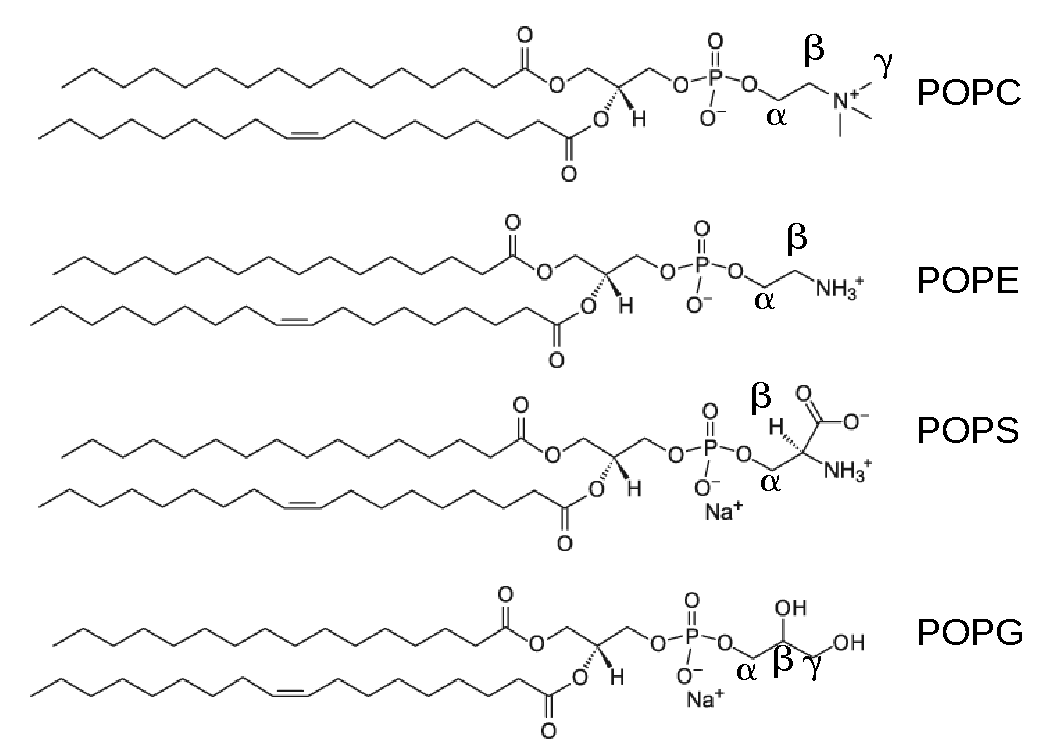
\includegraphics[width=9.0cm]{../Figs/lipids.pdf}
%  \caption{\label{lipids}
%    Chemical structures and labels for the headgroup carbons.
%  }
%\end{figure}



\section{Methods}
\subsection{Experimental C--H bond order parameters}
The headgroup and glycerol backbone C--H bond order parameter magnitudes and signs of POPE and POPG
were determined by measuring the chemical-shift resolved dipolar splittings
with a R-type Proton Detected Local Field (R-PDLF) experiment~\cite{dvinskikh04} and
%The corresponding order parameter signs were measured with a
S-DROSS experiments~\cite{gross97} using natural abundance $^{13}$C solid state NMR spectroscopy
as described previously \cite{ferreira13,ferreira16}.
%The experiments were done in a Bruker Avance III 400 spectrometer operating at a $^1$H Larmor frequency of 400.03 MHz.
%Magic angle spinning (MAS) of the sample was used at a frequency of 5.15 kHz (R-PDLF experiment) and 5 kHz (S-DROSS experiment).
%The following experimental setups were used.
POPE and POPG powder were purchased from Avanti polar lipids.
The NMR experiments were identical to our previous work~\cite{antila19}.
\todo{Is this enough and correct, or should we repeat some methods from the NMRlipidsIVps paper?}
The POPE experiments were recorded at 310~K and POPG experiments at 298~K, where the bilayers are in the liquid disordered phase \cite{marsh13}.


\subsection{Molecular dynamics simulations}

Molecular dynamics simulation data were collected using
the Open Collaboration method \cite{botan15}, with
the NMR\-lipids Project blog (\url{nmrlipids.blogspot.fi}) and
GitHub repository (\url{github.com/NMRlipids/NMRlipidsIVotherHGs})
as the communication platforms.
The simulated systems of pure PE and PG bilayers without additional ions
are listed in Tables \ref{systemsPE} and \ref{systemsPG},
and lipid mixtures with additional ions in Table~\ref{systemsMIX}.
Further simulation details are given in the SI, and
the simulation data are indexed in a
searchable database available at \url{www.nmrlipids.fi},
and in the NMRlipids/MATCH repository (\url{github.com/NMRlipids/MATCH}).

The C--H bond order parameters were calculated directly
from the carbon and hydrogen positions using the definition
\begin{equation}
S_{\rm CH}=\frac{1}{2}\langle 3\cos^2\theta -1 \rangle,
\end{equation}
where $\theta$ is the angle between the C--H bond and the membrane normal
(taken to align with $z$, with bilayer periodicity in the $xy$-plane).
Angular brackets denote average over all sampled configurations.
The order parameters were first calculated averaging over time separately
for each lipid in the system. The average and
the standard error of the mean were then calculated over different lipids.
Python programs that use the MDAnalysis library \cite{agrawal11,gowers16}
used for all atom simulations is available in Ref. \citenum{MATCHgit}
({\tt scripts/calcOrderParameters.py}). For united atom simulations, the trajectories
with hydrogens having ideal geometry were constructed first using either buildH program~\cite{buildH}
or ({\tt scratch/opAAUA\_prod.py}) in  Ref. \citenum{MATCHgit}, and the order parameters were
then calculated from these trajectories. This approach has been tested against trajectories
with explicit hydrogens and the deviations in order parameters are small \cite{buildH,piggot17}.\\
\todo{BuildH program is now cited with a direct link to the GitHub repo. I think that a release to Zenodo would be nice in the final publication.}\\
\todo{Maybe we should also shortly discuss here about the reasons for slight dependence of order parameter values on the method used to reconstruct hydrogens?}\\
The ion number density profiles were calculated using the {\tt gmx density} tool
of the Gromacs sofware package \cite{gromacsMANUAL}.

\begin{table*}[htb]
  %\begin{sidewaystable*}[!p]
  \centering
  \caption{List of MD simulations with PE lipids.
    % The salt concentrations calculated as [salt]=N$_{\rm c} \times$[water]\,/\,N$_{\rm w}$, where [water]\,=\,55.5~M.
    % these correspond the concentrations reported in the experiments by Akutsu et al.~\cite{akutsu81}.
    % The lipid force fields named as in our previous work~\cite{botan15}.
  }\label{systemsPE}
  \begin{minipage}[t]{\textwidth}
    \begin{tabular}{l c c r r r r r r c c}
      %\hline
      % some footnotes are not visible in typeset-MS (pdf)
      lipid/counter-ions & force field for lipids / ions  & NaCl (M) & \footnote{Number of lipid molecules with largest mole fraction}N$_{\rm l}$   &  \footnote{Number of water molecules}N$_{\rm w}$   & \footnote{Number of additional cations}N$_{\rm c}$   & \footnote{Simulation temperature}T (K)  & \footnote{Total simulation time}t$_{{\rm sim}}$(ns) & \footnote{Time used for analysis}t$_{{\rm anal}}$ (ns) &   \footnote{Reference for simulation files}files\\
      \hline
      POPE  & CHARMM36 \cite{??}           &0       & 144	& 5760  &0    & 310  & 500          & 400          & \cite{charmm36POPEfiles} \\
      POPE  & CHARMM36 \cite{??}           & 0      & 500       & 25000 & 0   &  310  & 500 & 100 & \cite{POPEcharmm} \\
      POPE  & CHARMM36 \cite{??}           & 0.11   & 500       & 25000 & 50  &  310  & 500 & 100 & \cite{POPEcharmm150mMNaCl} \\
      POPE  & CHARMM36ua \cite{??}         &0       & 336	& 15254 &0    & 310  & 2$\times$200 & 2$\times$100 & \cite{charmm36uaPOPEfiles}  \\
      \hline
      DPPE  & Slipids \cite{jambeck12b}    &0    & 288 	& 9386  &0    & 336  & 200 & 100 & \cite{slipidsDPPEfiles}  \\
      POPE  & Slipids \cite{jambeck12b} &0    & 336	& ?     &0    & 310  & 2$\times$200 &  2$\times$100 & \cite{slipidsPOPEfiles}  \\
      POPE  & Slipids \cite{jambeck12b}            & 0    & 500 & 25000 & 0   &  310  & 500 & 100 & \cite{POPEslipids} \\
      POPE  & Slipids / {\AA}qvist \cite{jambeck12b,aqvist90}  & 0.11 & 500 & 25000 & 50  &  310  & 500 & 100 & \cite{POPEslipids150mMNaCl} \\
      \hline
      DPPE  & GROMOS-CKP    \cite{??}      &0    & 128	& 3655  &0    & 342  & 2$\times$500 & 2$\times$400 & \cite{gromosCKPdppe} \\
      POPE  & GROMOS-CKP    \cite{??}      &0    & 128	& 3552  &0    & 313  & 2$\times$500 & 2$\times$400 & \cite{gromosCKPpope} \\
      POPE  & GROMOS-CKP    \cite{??}      &0    & 500	& 25000 &0    & 310  & 500 & 100 & \cite{gromosCKPpopeT310} \\
      POPE  & GROMOS-CKP    \cite{??}      &0.11 & 500	& 25000 &50   & 310  & 500 & 100 & \cite{gromosCKPpopeT310150mMNaCl} \\
      DOPE  & GROMOS-CKP    \cite{??}      &0    & 128	& 4789  &0    & 271  & 2$\times$500 & 2$\times$400 & \cite{gromosCKPdope} \\
      \hline
      POPE  & GROMOS 43A1-S3 \cite{??}     &0    & 128	& 3552     &0    & 313  & 2$\times$200 & 2$\times$100 & \cite{gromos43a1s3POPEfiles}  \\
      \hline
      POPE  & OPLS-UA vdW on H \cite{??}   &0    & 128	& 3328     &0    & 303  & 2$\times$200 & 2$\times$100 & \cite{OPLSuaWvdWPOPEfiles} \\
      POPE  & OPLS-UA \cite{??}            &0    & 128	& 3328     &0    & 303  & 2$\times$200 & 2$\times$100 & \cite{OPLSuaPOPEfiles} \\
      \hline
      POPE  & OPLS-MacRog \cite{rog16}     &0    & 144	& 5760     &0    & 310  & 500 & 350 & \cite{MacRogPOPEfiles} \\
      POPE  & OPLS-MacRog \cite{rog16}     &0    & 128	& 5120     &0    & 300  & 500 & 300 & \cite{MacRogPOPEfilesT300K} \\
      \hline
      POPE  & Berger-Vries \cite{??}       &0    & 128	& 3552  &0    & 303  & 2$\times$200 & 2$\times$100 & \cite{bergerPOPEfiles}  \\
      POPE  & Berger-largeH \cite{??}      &0    & 128	& 3552  &0    & 303  & 2$\times$200 & 2$\times$100 & \cite{berger2POPEfiles}  \\
      DOPE  & Berger-Vries \cite{??}       &0    & 128	& 4789  &0    & 271  & 2$\times$200 & 2$\times$100 & \cite{bergerDOPEfiles}  \\
      DOPE  & Berger-largeH \cite{??}      &0    & 128	& 4789  &0    & 271  & 2$\times$300 & 2$\times$100 & \cite{berger2DOPEfiles} \\ 
      \hline
      POPE             & LIPID17 \cite{gould18} & 0      & 500 & 25000 & 50  &  310  & 500 & 100 & \cite{POPElipid17} \\
      POPE             & LIPID17 \cite{gould18} & 0.11   & 500 & 25000 & 50  &  310  & 500 & 100 & \cite{POPElipid17150mMNaCl} \\
    \end{tabular}
  \end{minipage}
  %\end{sidewaystable*} 
  \todo{Citation for CHARMM36 PE?} \\
  \todo{Which ion model is used in \cite{POPEcharmm150mMNaCl}?} \\
  \todo{Citation for GROMOS-CKP?} \\
  \todo{Citation for GROMOS 43A1-S3?} \\
  \todo{Citation for OPLS-UA models?} \\
  \todo{Citations for Berger-* simulations?} \\
  \todo{LIPID17 simulations with correct dihedrals still coming}
\end{table*}

      \begin{table*}[htb]
  %\begin{sidewaystable*}[!p]
  \centering
  \caption{List of MD simulations with PG lipids.
    % The salt concentrations calculated as [salt]=N$_{\rm c} \times$[water]\,/\,N$_{\rm w}$, where [water]\,=\,55.5~M.
    % these correspond the concentrations reported in the experiments by Akutsu et al.~\cite{akutsu81}.
    % The lipid force fields named as in our previous work~\cite{botan15}.
  }\label{systemsPG}
  \begin{minipage}[t]{\textwidth}
    \begin{tabular}{l c c r r r r r r c c}
      %\hline
      % some footnotes are not visible in typeset-MS (pdf)
      lipid/counter-ions & force field for lipids / ions & NaCl (M) &  \footnote{Number of lipid molecules with largest mole fraction}N$_{\rm l}$   &  \footnote{Number of water molecules}N$_{\rm w}$   & \footnote{Number of additional cations}N$_{\rm c}$  & \footnote{Simulation temperature}T (K)  & \footnote{Total simulation time}t$_{{\rm sim}}$(ns) & \footnote{Time used for analysis}t$_{{\rm anal}}$ (ns) &   \footnote{Reference for simulation files}files\\
      \hline
      POPG/K$^+$  & CHARMM36 \cite{??} \todoi{Correct citation for CHARMM POPG}    &0         & 118& 4110   &0    & 298  & 100 & 100 & \cite{CHARMM36popg}  \\
      POPG             & CHARMM36 \cite{??}        & 0.11           & 500 & 25000 & 49  &  310  & 500 & 100 & \cite{POPGcharmm150mMNaCl} \\
      POPG             & CHARMM36 \cite{??}        & 0              & 500 & 25000 & 0   &  310  & 500 & 100 & \cite{POPGcharmm} \\
      \hline
      POPG/Na$^+$  & Slipids / {\AA}qvist \cite{jambeck13,aqvist90}    &0         & 288 	& 10664   &0     & 298  & 250 & 100 & \cite{slipidsPOPGfiles} \\
      DPPG/Na$^+$  & Slipids / {\AA}qvist \cite{jambeck13,aqvist90}    &0         & 288 	& 11232  &0     & 314  & 200 & 100 & \cite{slipidsDPPGfiles} \\
      DPPG/Na$^+$  & Slipids / {\AA}qvist \cite{jambeck13,aqvist90}    &0         & 288 	& 11232   &0     & 298  & 400 & 100 & \cite{slipidsDPPGfilesT298K} \\
      POPG         & Slipids / {\AA}qvist \cite{jambeck13,aqvist90}    & 0    & 500 & 25000 & 0  &  310  & 500 & 100 & \cite{POPGslipids} \\
      POPG         & Slipids / {\AA}qvist \cite{jambeck13,aqvist90}    & 0.11    & 500 & 25000 & 49  &  310  & 500 & 100 & \cite{POPGslipids150mMNaCl} \\
      \hline
      POPG             & LIPID17 / Dang \cite{gould18,smith94}         & 0              & 500 & 25000 & 0   &  310  & 500 & 100 & \cite{POPGlipid17} \\
      POPG             & LIPID17 \cite{??}         & 0.11           & 500 & 25000 & 49  &  310  & 500 & 100 & \cite{POPGlipid17150mMNaCl} \\
      \hline
      POPG             & GROMOS-CKP \cite{??}         & 0              & 500 & 25000 & 0  &  310  & 500 & 100 & \cite{POPGgromosCKP} \\
      POPG             & GROMOS-CKP \cite{??}         & 0.11           & 500 & 25000 & 49 &  310  & 500 & 100 & \cite{POPGgromosCKP150mMNaCl} \\
    \end{tabular}
  \end{minipage}
  % \end{sidewaystable*}
  \todo{Citations and ion model for CHARMM36?} \\
  \todo{Lipid17 simulation with correct dihedral potentials still coming.} \\
  \todo{Citation and ion model for GROMOS-CKP?}
\end{table*}

\begin{table*}[htb]
  %\begin{sidewaystable*}[!p]
  \centering
  \caption{List of MD simulations with PE and PG lipids mixed with PC.
    % The salt concentrations calculated as [salt]=N$_{\rm c} \times$[water]\,/\,N$_{\rm w}$, where [water]\,=\,55.5~M.
    % these correspond the concentrations reported in the experiments by Akutsu et al.~\cite{akutsu81}.
    % The lipid force fields named as in our previous work~\cite{botan15}.
  }\label{systemsMIX}
  \begin{minipage}[t]{\textwidth}
    \begin{tabular}{l c c r r r r r r c c}
      %\hline
      % some footnotes are not visible in typeset-MS (pdf)
      lipid/counter-ions & force field for lipids / ions & NaCl (M) & CaCl$_2$\,(M) &  \footnote{Number of lipid molecules with largest mole fraction}N$_{\rm l}$   &  \footnote{Number of water molecules}N$_{\rm w}$   & \footnote{Number of additional cations}N$_{\rm c}$  & \footnote{Simulation temperature}T (K)  & \footnote{Total simulation time}t$_{{\rm sim}}$(ns) & \footnote{Time used for analysis}t$_{{\rm anal}}$ (ns) &   \footnote{Reference for simulation files}files\\
      \hline
      POPC                   & CHARMM36 \cite{??}        & 0.11      & 0  & 500     & 25000 & 48  &  310  & 500 & 100 & \cite{POPCcharmm150mMNaCl301K}  \\
      POPC:POPG (7:3)        & CHARMM36 \cite{??}        & 0.11      & 0  & 350     & ?     & ?   &  310  & 500 & 100 & \cite{POPC7POPG1charmm36NaCl}  \\
      POPC:POPG (1:1)/K$^+$  & CHARMM36 \cite{??}        &0          & 0  & 250:250 & 18158 & 0   &  298  & 200 & 200 & \cite{CHARMM36POPCPOPG5050} \\ 
      POPC:POPG (1:1)        & CHARMM36 \cite{??}        &0          & 0.34 \todoi{Concentration calculated based in total amount of calcium ions. This may not be reasonable due to the lack of counterions.}  & 250:250 & 20798 & 128 &  298  & 200 & 200 & \cite{CHARMM36POPCPOPG5050150mMCaCl} \\
      POPC:POPG (1:1)        & CHARMM36 \cite{??}        &0          & 1.36  \todoi{Concentration calculated based in total amount of calcium ions. This may not be reasonable due to the lack of counterions.} & 250:250 & 18114 & 445  &  298  & 200 & 200 & \cite{CHARMM36POPCPOPG50501000mMCaCl} \\
      POPC:POPG (4:1)/K$^+$  & CHARMM36 \cite{??}        &0          & 0  & 400:100 & 18664 & 0  &  298  & 200 & 200 & \cite{CHARMM36POPCPOPG4010} \\
      POPC:POPG (4:1)/K$^+$  & CHARMM36 \cite{??}        &0          & 1.0 \todoi{Concentration calculated based in total amount of calcium ions. This may not be reasonable due to the lack of counterions.} & 400:100 & 18647 & 419  &  298  & 200 & 200 & \cite{CHARMM36POPCPOPG40101000mMCaCl} \\
      \hline
      POPC             & CHARMM36 \cite{??}        &0          & 0  & 256 & 8704 & 0  &  300  & 300 & 250 & \cite{POPCcharmm300K} \\
      POPC:POPE (1:1)  & CHARMM36 \cite{??}        &0          & 0  & 128 & 8704 & 0  &  300  & 300 & 250 & \cite{POPC1POPE1charmm36} \\
      \hline
      POPC             & OPLS-MacRog \cite{rog16}     &0          & 0  & 128 & 5120 & 0  &  300  & 500 & 300 & \cite{POPCmacrog300K} \\
      POPC:POPE (1:1)  & OPLS-MacRog \cite{rog16}     &0          & 0  & 128 & 5120 & 0  &  300  & 500 & 300 & \cite{POPC1POPE1macrogT300K} \\
      \hline
      POPC             & Slipid \cite{jambeck12b}     &0          & 0  & 512 & 23943 & 0  &  300  & 170 & 100 & \cite{POPCslipid300K} \\
      POPC:POPE (1:1)  & Slipid \cite{jambeck12b}     &0          & 0  & 128 & 5120 & 0  &  300  & 500 & 300 & \cite{POPC1POPE1slipidT298K} \\
     \hline
      POPC                   & GROMOS-CKP / ?? \cite{??,??}  & 0         & 0  & 500     & 25000 & 0   &  310  & 500 & 100 & \cite{POPCgromosCKPT310K}  \\
      POPC:POPG (7:3)        & GROMOS-CKP / ?? \cite{??,??}  & 0         & 0  & 350:150 & 25000 & 0   &  310  & 500 & 100 & \cite{POPC7POPG3gromosCKPT310K} \\
     \hline
      POPC                   & Slipid / {\AA}qvist \cite{jambeck12b,aqvist90}  & 0         & 0  & 500     & 25000 & 0   &  310  & 500 & 100 & \cite{POPCslipid301K}  \\
      POPC:POPG (7:3)        & Slipid / {\AA}qvist \cite{jambeck12b,aqvist90}  & 0         & 0  & 350:150 & 25000 & 0   &  310  & 500 & 100 & \cite{slipidPOPC70POPG30T310K} \\
      POPC:POPG (1:1)        & Slipid / Dang \cite{jambeck12b,jambeck2012another,smith94,dang06} & 0         & 0  & 128:128 & 12800 & 0   &  298  & 500 & 400 & \cite{slipidPOPC50POPG50T298K} \\
      POPC:POPG (1:1)        & Slipid / Dang \cite{jambeck12b,jambeck2012another,smith94,dang06} & 0         & 0.1  & 128:128 & 12800 & 23  &  298  & 500 & 400 & \cite{slipidPOPC50POPG50T298K} \\
      POPC:POPG (1:1)        & Slipid / Dang \cite{jambeck12b,jambeck2012another,smith94,dang06} & 0         & 0.2  & 128:128 & 12800 & 46  &  298  & 1500 & 500 & \cite{slipidPOPC50POPG50T298K} \\
      POPC:POPG (1:1)        & Slipid / Dang \cite{jambeck12b,jambeck2012another,smith94,dang06} & 0         & 0.5  & 128:128 & 12800 & 115 &  298  & 1500 & 500 & \cite{slipidPOPC50POPG50T298K} \\
      POPC:POPG (1:1)        & Slipid / Dang \cite{jambeck12b,jambeck2012another,smith94,dang06} & 0         & 1.0  & 128:128 & 12800 & 230 &  298  & 1500 & 500 & \cite{slipidPOPC50POPG50T298K} \\
      
      \hline
      POPC:POPG (4:1)        & Lipid17 / Dang \cite{gould18,smith94,dang06}   &0          & 0  & 350:88 & 26265 & 0  &  298  & 400 & 350 & \cite{Lipid17POPCPOPG8020} \\
      POPC:POPG (4:1)        & Lipid17 / Dang \cite{gould18,smith94,dang06}        &0          & 0.1& 350:88 & 26124 & 47 &  298  & 400 & 150 & \cite{Lipid17POPCPOPG8020100mMCaCl} \\
      POPC:POPG (4:1)        & Lipid17 / Dang \cite{gould18,smith94,dang06}        &0          & 1.0& 350:88 & 24840 & 475 &  298  & 1200 & 200 & \cite{Lipid17POPCPOPG80201000mMCaCl} \\
      POPC:POPG (1:1)        & Lipid17 / Dang \cite{gould18,smith94,dang06}        &0          & 0  & 150:150 & 31572 & 0  &  298  & 320 & 200 & \cite{Lipid17POPCPOPG5050} \\
      POPC:POPG (1:1)        & Lipid17 / Dang \cite{gould18,smith94,dang06}     &0          & 0.1& 150:150 & 31401 & 57 &  298  & 720 & 198 & \cite{Lipid17POPCPOPG5050100mMCaCl} \\
      POPC:POPG (1:1)        & Lipid17 / Dang \cite{gould18,smith94,dang06}        &0          & 1.0& 150:150 & 29865 & 569 &  298  & 720 & 200 & \cite{Lipid17POPCPOPG50501000mMCaCl} \\
      \hline
      POPC             & Berger \cite{??} \todoi{This is probable not plain berger, correct force filed should be described.}  &0  & 0  & 256 & 10240 & 0  &  300  & 300 & 200 & \cite{POPCberger300K} \\
      POPC:POPE (1:1)  & Berger \cite{??}  \todoi{This is probable not plain berger, correct force filed should be described.} &0          & 0  & 128 & 11008 & 0  &  300  & 300 & 200 & \cite{POPC1POPE1berger} \\
      POPC:DOPE (1:1)  & Berger \cite{??}  \todoi{This is probable not plain berger, correct force filed should be described.}         &0          & 0  & 128 & 10240 & 0  &  300  & 300 & 200 & \cite{POPC1DOPE1berger} \\
     \hline
      DOPC             & Berger \cite{??}  \todoi{This is probable not plain berger, correct force filed should be described.}         &0          & 0  & 256 & 11008 & 0  &  300  & 300 & 200 & \cite{DOPCberger300K} \\
      DOPC:DOPE (1:1)  & Berger \cite{??}   \todoi{This is probable not plain berger, correct force filed should be described.}        &0          & 0  & 128 & 11008 & 0  &  300  & 300 & 200 & \cite{DOPC1DOPE1berger} \\
    \end{tabular}
  \end{minipage}
  %\end{sidewaystable*}
  \todo{New CHARMM simulations are still to be ran.} \\
  \todo{Citation and ion model for GROMOS-CKP?} \\
  \todo{Citation and description for ''Berger'' model?}
\end{table*}

\clearpage
\section{Results and Discussion}

\subsection{Headgroup and glycerol backbone order parameters of POPE and POPG from $^{13}$C NMR}
Absolute values of the headgroup and glycerol backbone order parameters from PE and PG lipids are measured
previously using $^2$H NMR~\cite{seelig76,gally81,wohlgemuth80,borle85}. Because also the order parameter
signs bear essential information about the lipid structures \cite{botan15,ollila16}, we measured the
magnitudes and signs of POPE and POPG C--H bond headgroup and glycerol backbone order parameter in liquid phase
using the 
%order parameters The order parameters for the glycerol backbone and headgroup s were determined
2D-RPDLF and S-DROSS experiments, as described previously \cite{ferreira13,ferreira16,antila19}.
For POPE, the glycerol backbone and $\alpha$-carbon peaks in INEPT spectra were assigned based on
previously measured POPC spectra~\cite{ferreira13} and
the $\beta$-carbon peak was assigned based on $^{13}$C chemical shift table for amines available
at \url{https://www.chem.wisc.edu/areas/reich/nmr/c13-data/cdata.htm} (Fig. \ref{POPEspectra}).
For POPG, the glycerol backbone peaks in INEPT spectra were assigned based on
previously measured POPC spectra~\cite{ferreira13}, while $\alpha$ and  $\gamma$-carbon peaks
\todo{How were these assigned?} (Fig. \ref{POPGspectra}). The numerical value of the $\beta$-carbon
order parameter could not be determined, because its peak overlapped with the g$_2$ peak from glycerol backbone in POPG.
However, the order parameter of $\beta$-carbon is expected to be clearly smaller than for g$_2$
based on previous $^2$H NMR measurements \cite{wohlgemuth80,gally81,borle85}.
Therefore, the beginning of the S-DROSS curve gives the sign for g$_2$ order parameter and end for $\beta$ (Fig. \ref{POPGspectra} (E)).
This is confirmed with SIMPSON calculations using negative value for g$_2$ and positive value for $\beta$ order parameter (Fig. \ref{POPGsimpson}).
\todo{Details to be checked by Tiago}.

As discussed previously for PC and PS headgroups \cite{ollila16,antila19}, also 
the headgroup and glycerol backbone order parameters of PE and PG are essentially independent of 
acyl chain composition, and therefore manifest mainly headgroup chemistry (Fig. \ref{HGorderParameters}).
The glycerol backbone order parameters are similar for all the lipids, although they move slightly toward
positive values (closer to zero) in the order PC $<$ PE $<$ PS $<$ PG. 
Also the headgroup order parameters of PC lipids are close PE, althought the latter gives systematically
slightly more positive values (Fig. \ref{HGorderParameters}).
% These could be explained with slightly larger temperature in PE measurements, except for the $\alpha$-carbon with the positive sign, for which the
% more positive value is farther away from zero.
The $\alpha$-carbon order parameter of PG is similar to PE and PG, while the positive value of $\beta$-carbon
is distinct from the other lipids. Notably, this difference was not observed in previous $^2$H NMR experiments,
because absolute value of $\beta$-carbon order parameter is similar in PG, PE and PC lipids and the order parameter
signs were not measured~\cite{wohlgemuth80,gally81,borle85}.

In conclusion, the order parameter experiments suggest that the glycerol backbone conformations in all lipids
and the headgroup conformations in PC and PE lipids are relatively similar, while 
PS and PG headgropus exhibit distinct conformational sampling.
The details of sampled conformation are difficult to deduce from order parameters only,
but the distinct headgroup order parameters
of PS lipids are previously related to the more rigid structure of the headgroup~\cite{browning80,buldt81,antila19}.

\begin{figure}[]
  \centering
  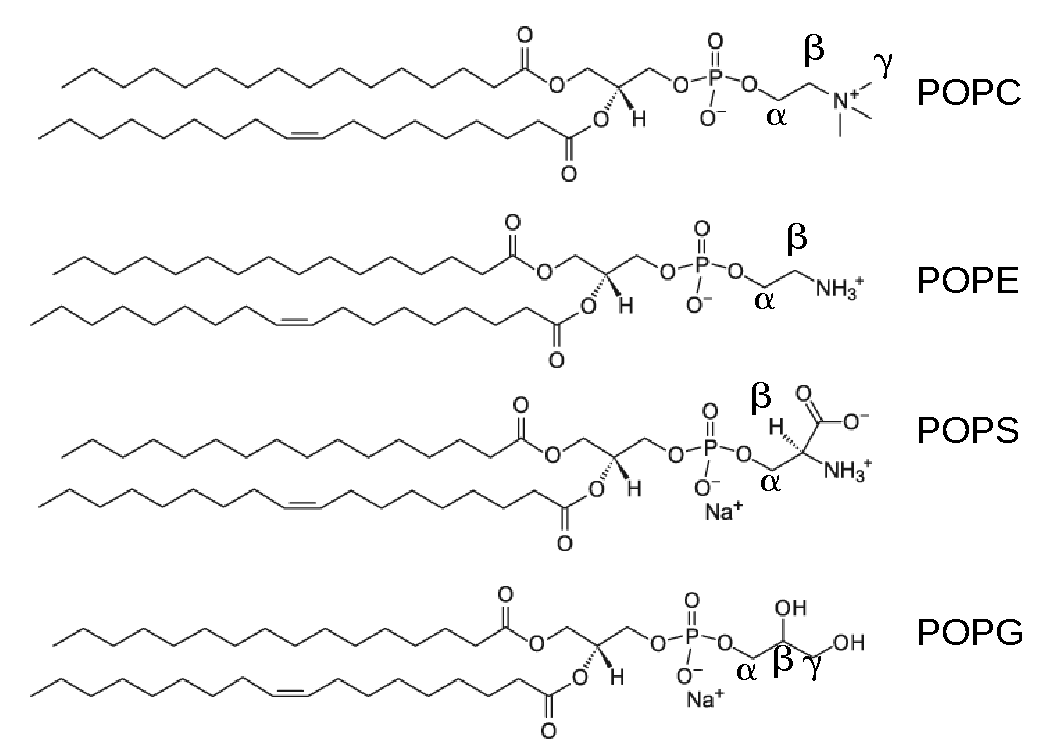
\includegraphics[width=9.0cm]{../Figs/lipids.pdf}
  \includegraphics[width=9.0cm]{../Figs/HGorderparametersPCPSPEPG.eps}
  \caption{\label{HGorderParameters}
    (top) Chemical structure of different lipids.
    (bottom) Headgroup and glycerol backbone order parameters
    from different experiments in lamellar liquid disordered phase.
    The values and signs for POPE (310~K) and POPG (298~K)
    measured in this work, and for POPS (298~K) \cite{antila19} and POPC (300~K) \cite{ferreira13,ferreira16}
    previously using $^{13}$C NMR. The literature values for
    DOPS with 0.1M of NaCl (303~K) \cite{browning80},
    POPG with 10nM PIPES (298~K) \cite{borle85},
    DPPG with 10mM PIPES and 100mM NaCl (314~K) \cite{wohlgemuth80}, 
    DPPE (341~K) \cite{seelig76},
    E.coliPE and E.coliPG (310~K) \cite{gally81}
    are measured using $^2$H NMR. The signs from $^{13}$C NMR are used also for the literature values.
  }
  \todo{The bottom figure could be clarified as Fig. 2 in the NMRlipids IVps paper.}
\end{figure}


\subsection{Headgroup and glycerol backbone of POPE and POPG in MD simulations}
Headgroup and glycerol backbone order parameters of PE and PG lipids
show wide variation between different force fields
and none of the force fields reproduce all values within experimental error bars.
(Figs. \ref{HGorderParametersPE} and \ref{HGorderParametersPOPG}),
as observed previously also for PC and PS lipids \cite{botan15,antila19}.
%The Slipid simulations were able to capture the essential differences between PC and PS lipid
%headgroups \cite{antila19}, but this is not the case for PE and PG lipids.
The poor performance of headgroup order parameters in Berger model can be probably explained by
ring like structures seen in Fig. 6 in Ref. \citenum{mukhopadhyay04}, which is a typical feature
for Berger based lipid force fields containing explicit hydrogen atoms in the head group \cite{zhao08,henin09,dahlberg10}.
The poor performance of glycerol backbone of Slipids simulations is systemically observed also
for other lipids in previous studies \cite{botan15,antila19}.
\todo{Should we comment more the relative quality of different force fields and/or make the subjective force field ranking figures?
https://github.com/NMRLipids/NMRlipidsIVPEandPG/issues/8}

\begin{figure}[]
  \centering
  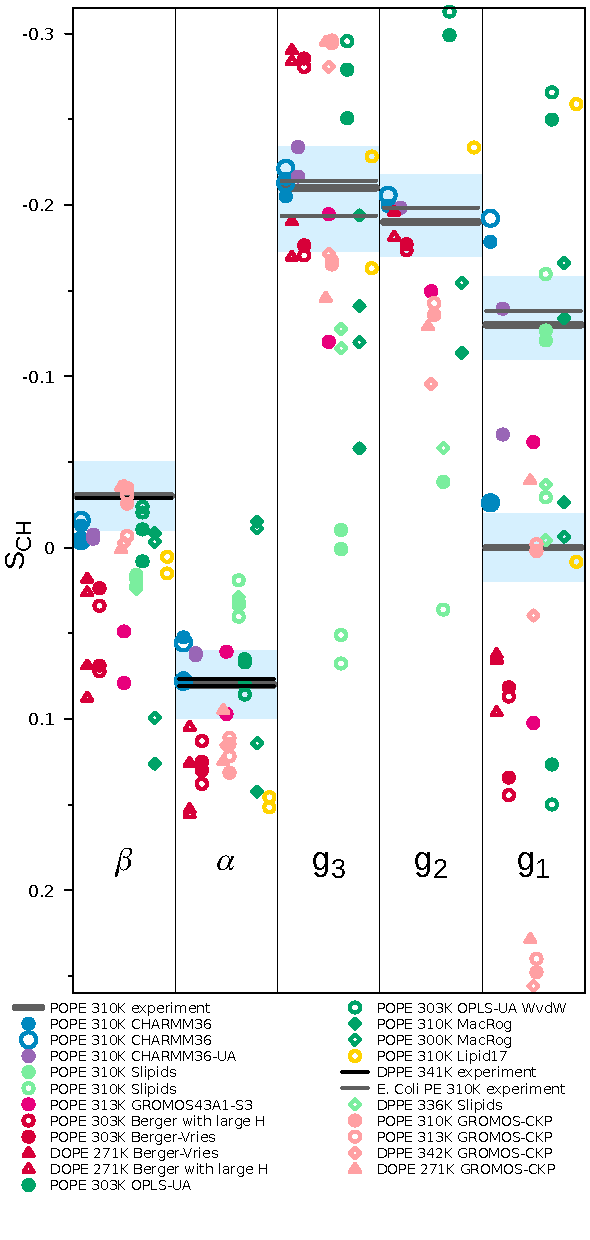
\includegraphics[width=9.0cm]{../Figs/HGorderparametersPE.pdf}
  \caption{\label{HGorderParametersPE}
    The headgroup and glycerol backbone order parameters of PE lipids
    from experiments (POPE and signs this work, DPPE from Ref.~\citenum{seelig76}
    and E.coliPE from Ref.~\citenum{gally81}) and simulations with different force fields.
  }
  \todo{This should be clarified as in NMRlipidsI and error bars should be added.
    Probably larger error bars for united atom models based on the report by Fuchs et al.
  } \\
\end{figure}

\begin{figure}[!h]
  \centering
  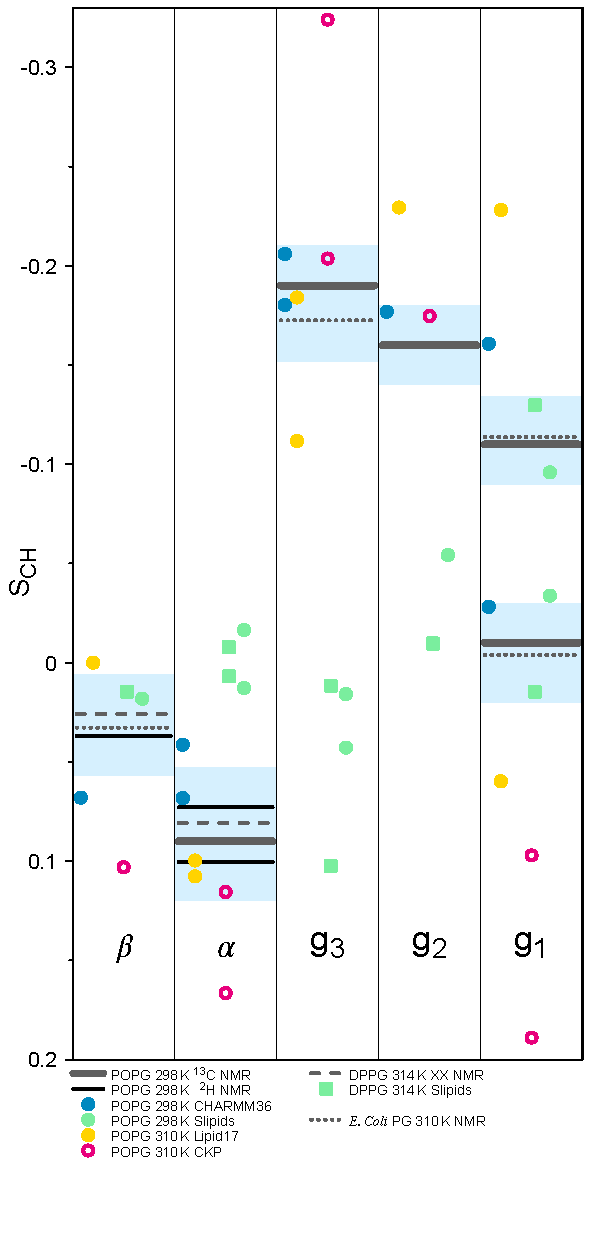
\includegraphics[width=9.0cm]{../Figs/HGorderparametersPG.pdf}
  \caption{\label{HGorderParametersPOPG}
    The headgroup and glycerol backbone order parameters of PG lipids
    from experiments (POPG and signs from this work and from Ref.~\citenum{borle85}, %contains 10mM of PIPES,
    DPPG with 100mM NaCl from Ref.~\citenum{wohlgemuth80},% contains 10mM PIPES and,
    and E.Coli PG results from Ref.~\citenum{gally81}).
    and simulations with different force fields.
  }
\end{figure}

Without further discussion about poorly performing force fields, we focus on more detailed analysis
of CHARMM36 simulations, which captures the essential differences between
PC, PS, PG and PE headroup order parameters  (Fig.~\ref{structures}) with the exception of $\beta$-carbon order parameter of PC
%give the best overall agreement with experiments for
%the headgroup and glycerol backbone order parameters of all PC, PS, PG and PE lipids in this and our previous
%studies \cite{botan15,antila19}. Even thought many order parameters in CHARMM36 simulations are
%not within the experimental error bars, it 
which is too negative when compared with PS or PE order parameter, or with experiments \cite{botan15}.
%As already pointed out in our previous study \cite{antila19},
Characteristic dihedral conformations in PS headgroup are asymmetric conformations
preferring gauche 270$^\circ$ conformations in N-C$_\beta$-C$_\alpha$-O$_\alpha$ and
%dihedral exhibits a more asymmetric angle distribution for PS, having largest probability being
%in , than for the PC headgroup.
C$_\beta$-C$_\alpha$-O$_\alpha$-P dihedrals. 
In PG headgroup, the O$_\beta$-C$_\beta$-C$_\alpha$-O$_\alpha$ dihedral (corresponding N-C$_\beta$-C$_\alpha$-O$_\alpha$ dihedral in other lipids)
is mostly in trans conformation, and C$_\beta$-C$_\alpha$-O$_\alpha$-P  has asymmetric tendency to be in
gauche 60$^\circ$ conformation. 
Main difference between PC and PE is the lower probability of trans state in C$_\beta$-C$_\alpha$-O$_\alpha$-P PC dihedral,
which could be a potential reason for the too negative $\beta$ headgroup order parameter in PC.

\begin{figure*}[!h]
  \centering
  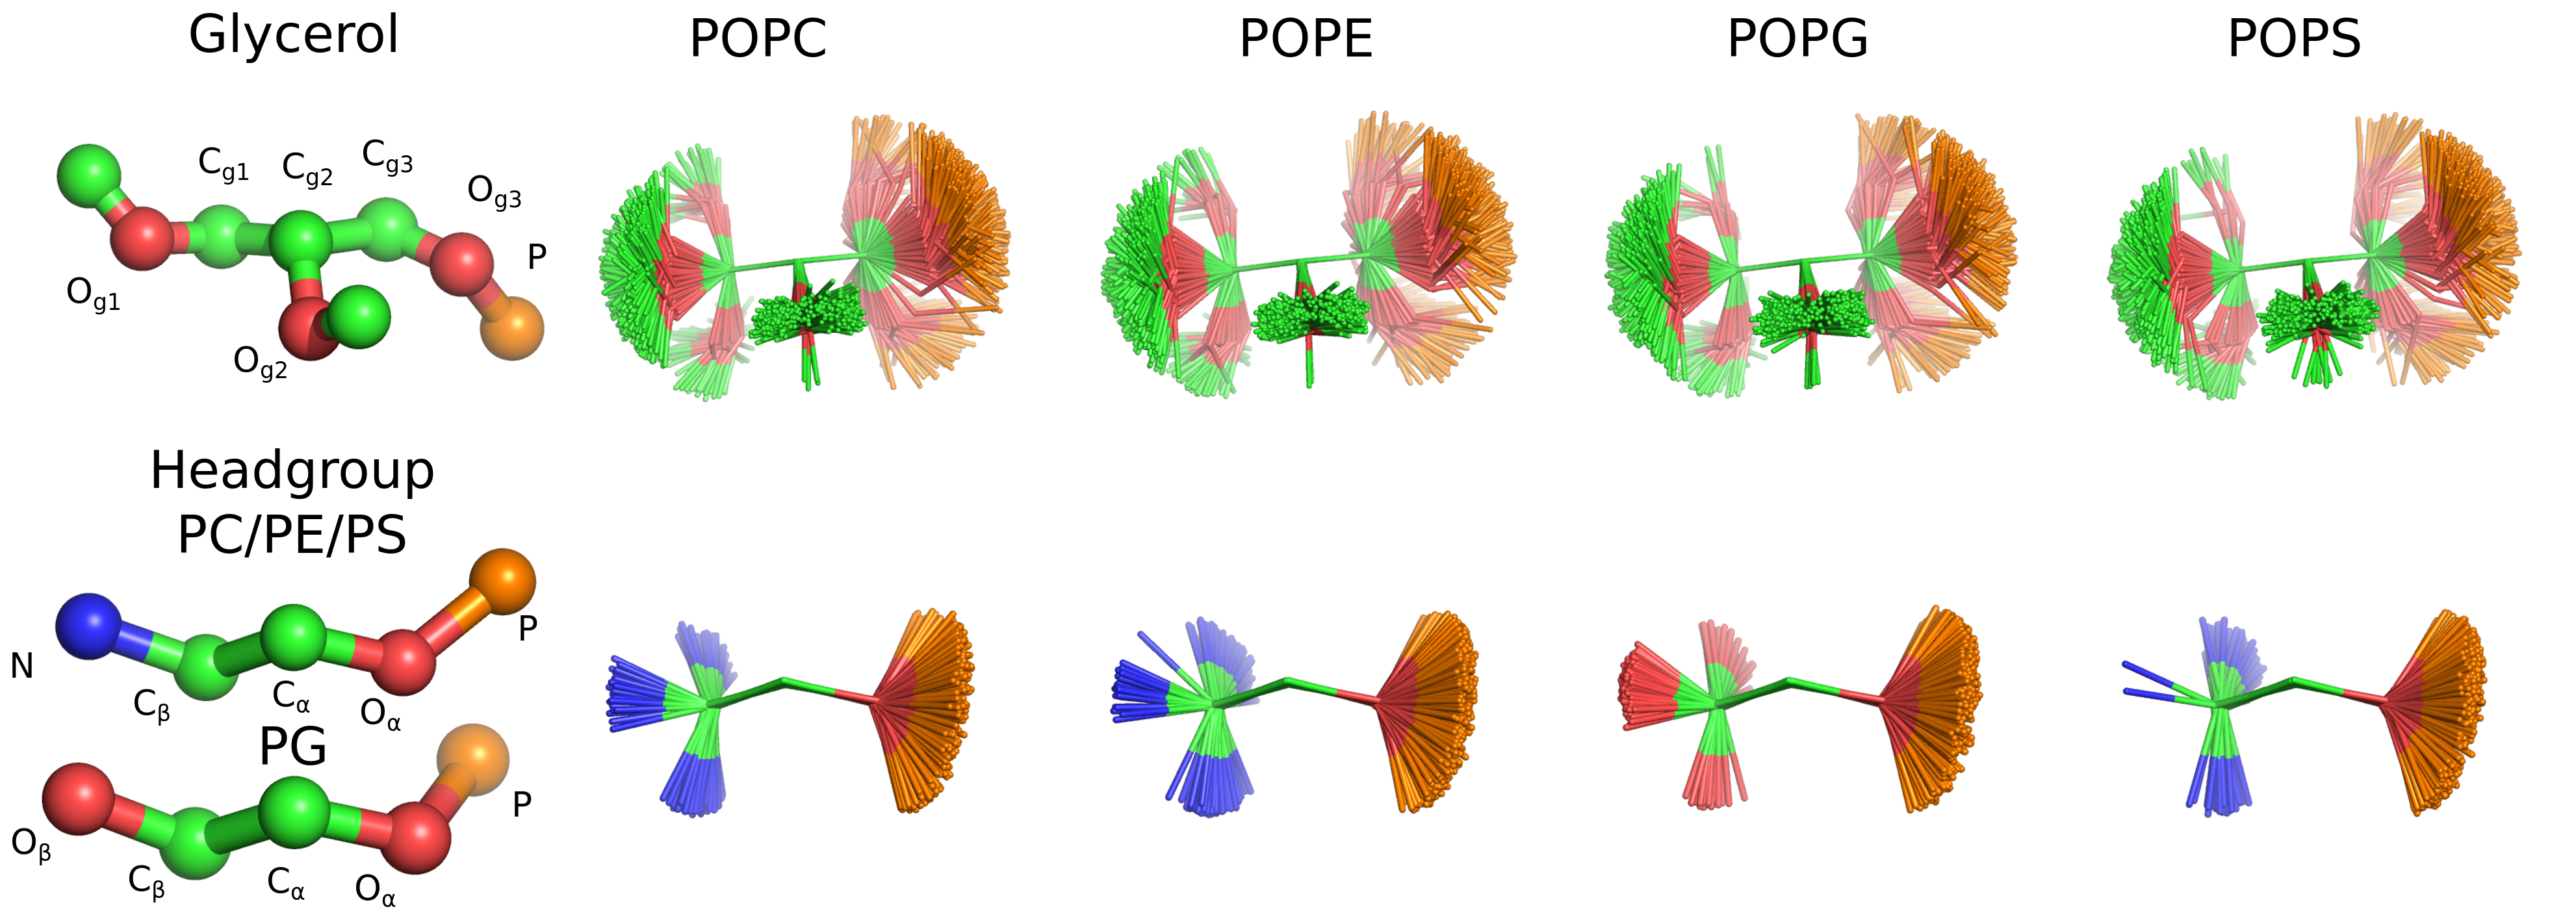
\includegraphics[width=18.0cm]{../Figs/PCPEPGPSstructures.png}
  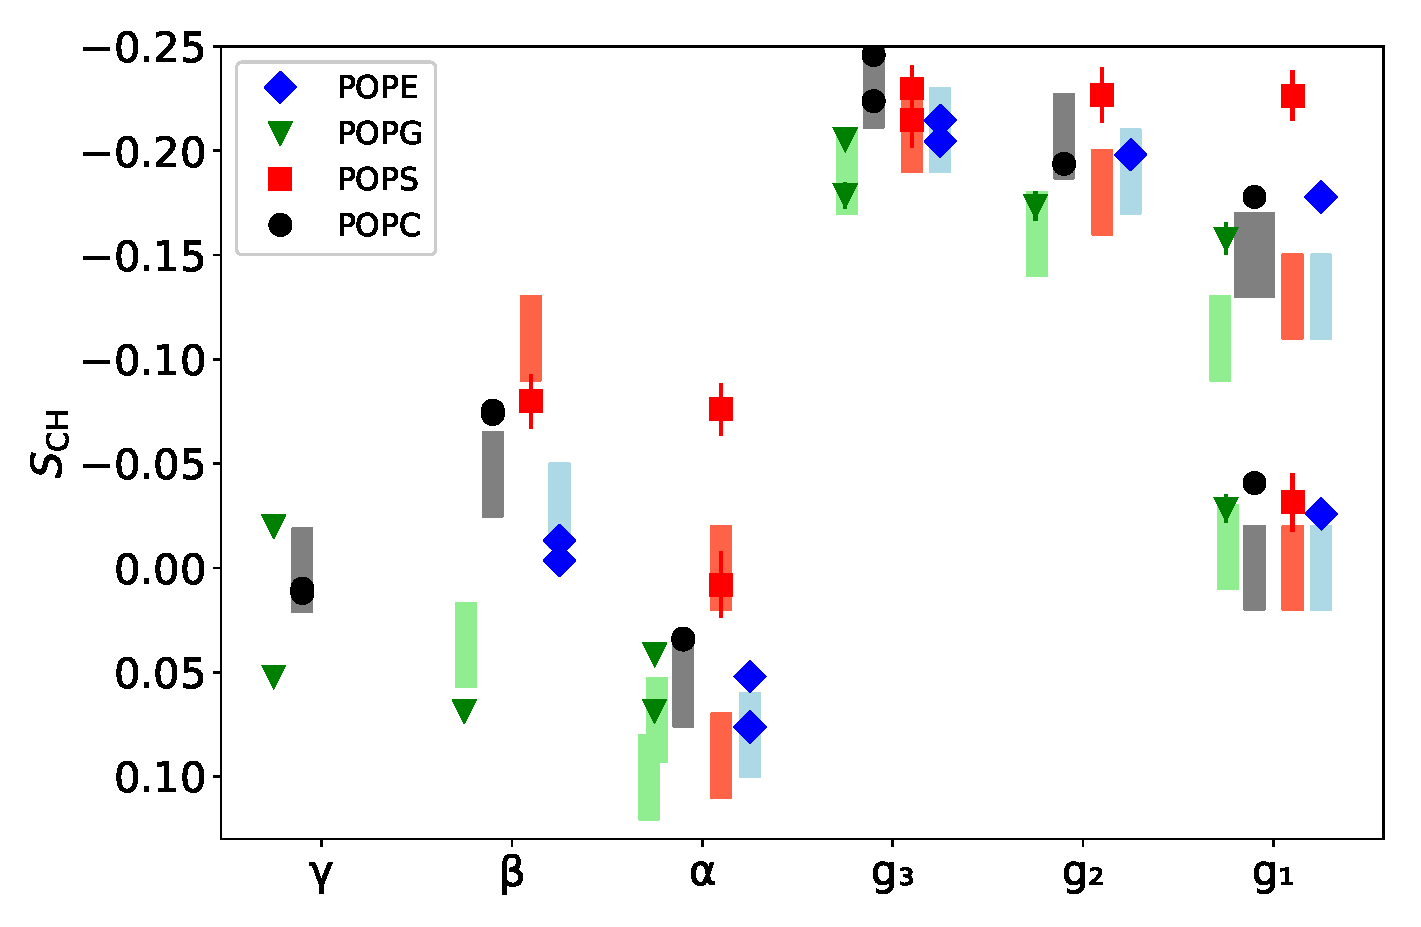
\includegraphics[width=8.0cm]{../Figs/CHARMMfromLIPIDS.eps}
  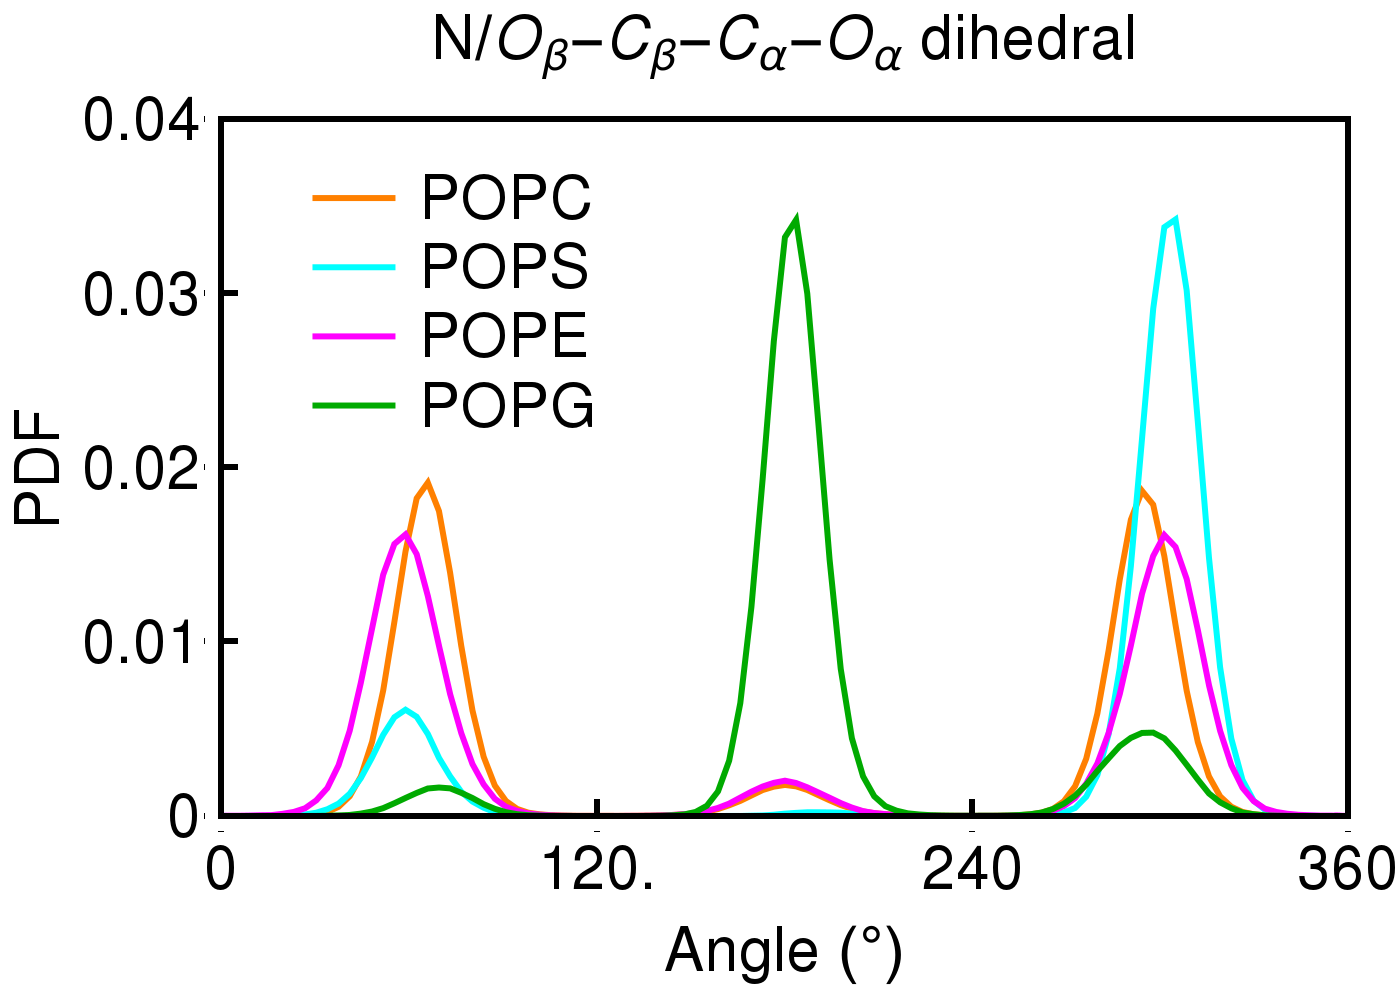
\includegraphics[width=8.0cm]{../Figs/PCPEPGPSdihedrals1.png}
  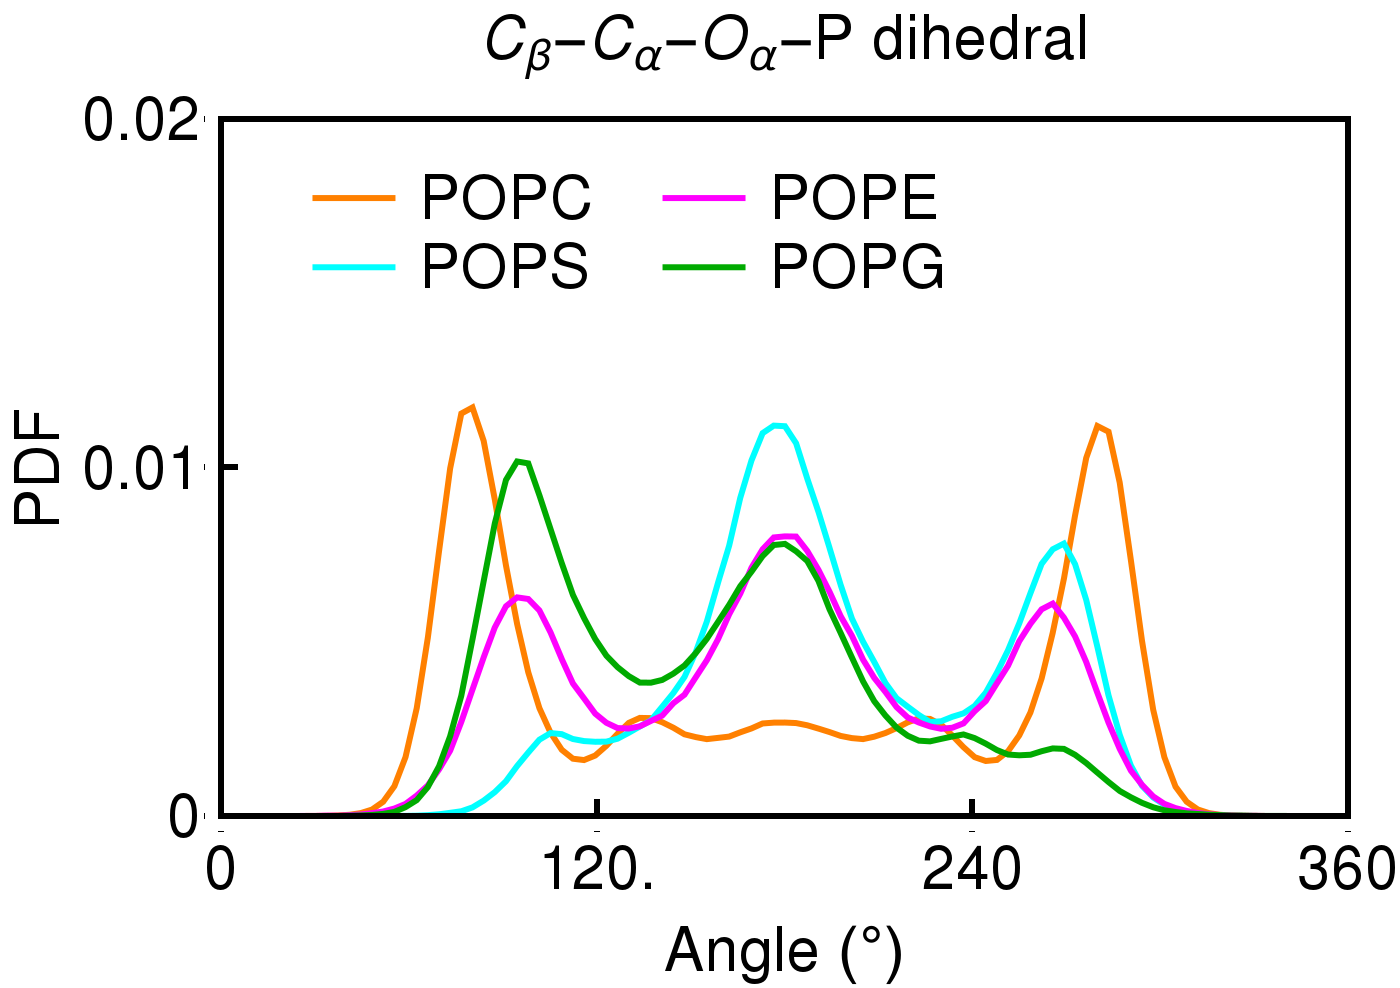
\includegraphics[width=8.0cm]{../Figs/PCPEPGPSdihedrals2.png}
  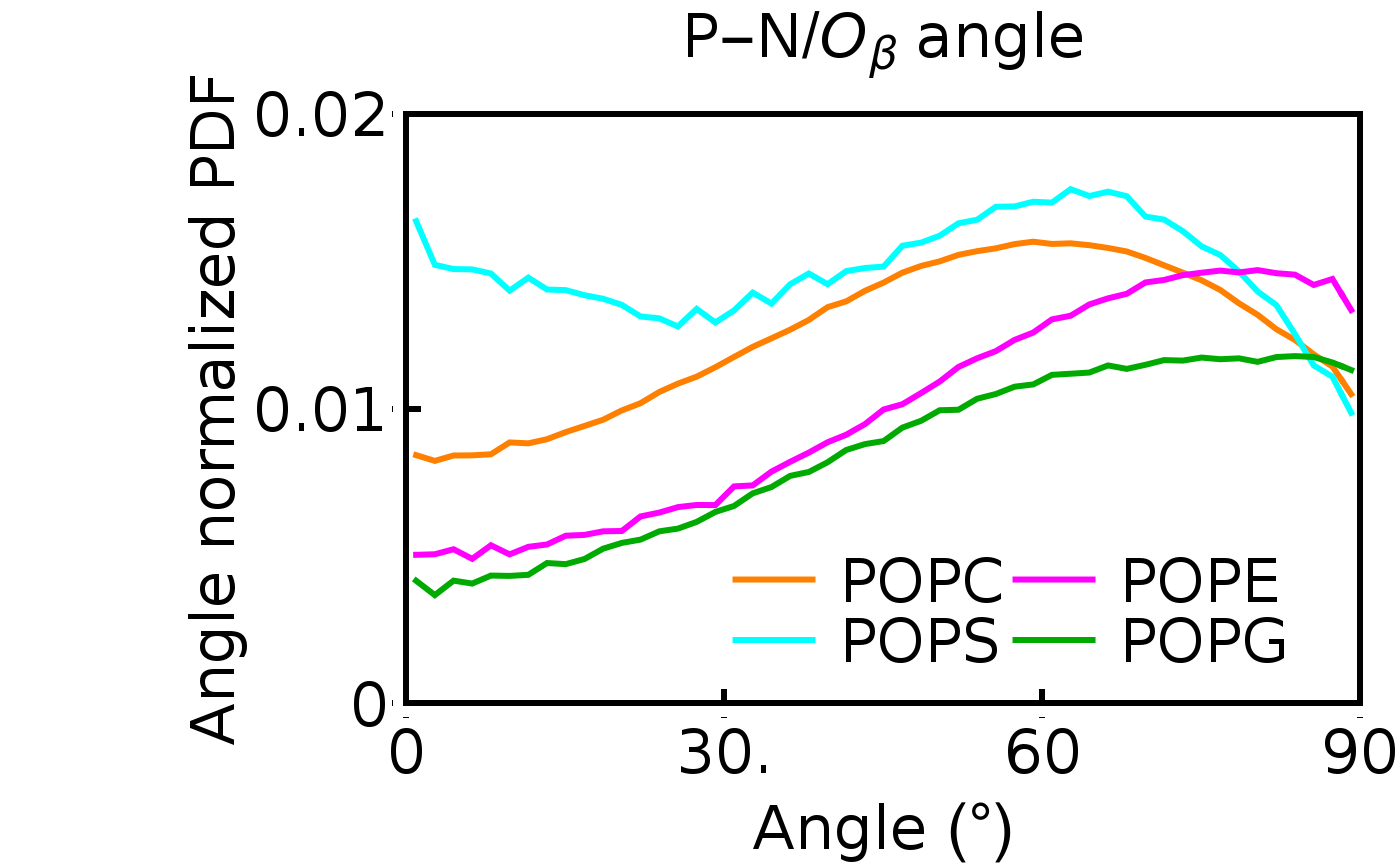
\includegraphics[width=8.0cm]{../Figs/HGtilt.png}
  \caption{\label{structures}
    Overlayed snapshots and dihedral angle distributions from CHARMM36 simulations of different lipids
    which give the best agreement with experiments.
  }
  \todo{The differences observed in dihedral distributions are not visible in the snapshot figures.} \\
  \todo{Why integral of the P-N angle distributions are not the same?} \\
  \todo{More detailed discussion of this figure is in https://github.com/NMRLipids/NMRlipidsIVPEandPG/issues/9} \\
\end{figure*}

\clearpage
\subsection{PC headgroup interactions with PE and PG}
\begin{figure*}[]
  \centering
  \includegraphics[width=16.0cm]{../Figs/HGorderparametersPCvsPEPG.eps}
  \caption{\label{HGorderparametersPCvsPEPG}
    Modulation of POPC headgroup order parameters with increasing amount of POPE (left) and POPG (right) in bilayer
    from experiments \cite{scherer87,macdonald87} and simulations with different force fields.
    Signs are determined as discussed in \cite{botan15,ollila16}.
  }
  %\todo{Simulation of CHARMM36 at 298K should be maybe rerun with Gromacs 5.}
\end{figure*}

In experiments, the PC headgroup order parameters increase
with the addition of negatively charged PG or PS lipids, but
are not affected by the addition of zwitterionic PE and SM lipids
or cholesterol (Fig.~\ref{HGorderparametersPCvsPEPG}).
This can be explained by the electrometer concept, which suggests that the 
headgroup dipole tilts more parallel to the membrane plane upon addition of
negative charge to the membrane~\cite{seelig87, scherer87,antila18}.
The response of PC headgroup order parameters to PE by the tested CHARMM36 and
Berger-OPLS force fields, although CHARMM36 slightly overestimates the changes (Fig.~\ref{HGorderparametersPCvsPEPG}).
The good performance of Berger-OPLS simulations is notable because the response of headgroup order parameters
to cholesterol was significantly overestimated by the Berger/Höltje force field in our previous work \cite{botan15}.
\todo{This is text by P. Fuchs, copied from the blog. \\
Area results in nm$^2$, the error is $<=$ 0.003 nm$^2$ \\
- pure POPC \\
CHARMM36: 0.624 \\
Berger : 0.649 \\
- POPC/POPE 50:50 \\
CHARMM36 : POPC 0.609, POPE 0.557 \\
Berger-hacked: POPC 0.637, POPE 0.632 \\
----- \\
One can see that CHARMM 36 predicts a drop in the area on going from pure POPC to POPC/POPE 50:50. This means that POPC pack tightly to POPE. 
In contrast, the values for Berger are not that changed. 
The POPE value predicted by CHARMM 36 (in the mixture POPC/POPE 50:50) is much smaller than that predicted by Berger.\\
-------\\
The experimental acyl chain order parameters for POPE \cite{pare98} seem larger than reported for POPC \cite{ferreira13},
which supports the more condensed PE bilayer.
This is interesting, but not exactly the core message of the manuscript.
Maybe we should mention this very briefly? For example, we could just report the areas per lipid (without distinguishing PC and PE)
and mention the difference between CHARMM36 and Berger. I have opened an issue for this: https://github.com/NMRLipids/NMRlipidsIVPEandPG/issues/7
}



None of the force fields fully reproduces the PC headgroup order parameter response to the increasing amount of
PG, which may be related to the counterion binding affinity (see also the next section) \cite{antila19}.
In all force fields except Slipids, the order parameters of different
hydrogens attached to the $\alpha$-carbon are responsing differently when mixed with PE or PG lipids
\todo{Maybe we should figure out what is the reason for this? \\
  Maybe we should analyze the P-N vector angle from different simulations? \\
  https://github.com/NMRLipids/NMRlipidsIVPEandPG/issues/10}.

For $\beta$-carbon order parameter in PG headgroup, experiments report
mild increase \cite{macdonald87} or no change~\cite{borle85} upon addition 
of PC lipids (Fig. \ref{HGorderparametersPGvsPCchange}). 
Simulations with all the tested force fields give only very small changes also for
the $\alpha$-carbon order parameter (Figs. \ref{HGorderparametersPGvsPC} and \ref{HGorderparametersPGvsPCchange}). 
Therefore, the simulations are generally in line with experiments, suggesting that the
interactions with PC do not essentially effect the PG headgroup structure.
This suggests that the interactions between PG and PC headgroups are captured better in
simulations than for PS headgroup, where
all the force fieds significantly overestimated the structural response of PS headgroup
to the interactions with PC lipids \cite{antila18}.
\begin{figure}[]
  \centering
  \includegraphics[width=8.0cm]{../Figs/HGorderparametersPGvsPCchange.eps}
  \caption{\label{HGorderparametersPGvsPCchange}
    Modulation of PG lipid headgroup order parameters with the increasing amount of PC in lipid bilayer
    from experiments \cite{borle85,macdonald87} and simulations with different force fields.
  }
\end{figure}




\clearpage
\subsection{Sodium binding to PE and PG lipid bilayers}
Sodium binding affinity to PE lipids has not been measured experimentally,
but large differences to PC would be surprising. 
In simulations, the sodium binding affinity to POPE depends on the used force field (Fig. \ref{NAdensPE}),
but lesser extend than reported previously for PC~\cite{catte16}.
\todo{This will be finished once we have all the simulation details and Lipid17 simulations with correct dihedrals from issue https://github.com/NMRLipids/NMRlipidsIVPEandPG/issues/12},
Because some simulation and ion parameters are not identical with the previous work~\cite{catte16},
we compare POPE results to the POPC simulations ran with identical parameters (Fig. \ref{NAdensPC}).
In Lipid17 with the strongest sodium binding affinity to POPE,
the binding affinity is approximately similar to POPC.
Slipids and CHARMM36 exhibit slightly, and
GROMOS-CKP subtantially weaker binding to POPE than to POPC.
%The Lipid17 exhibits stronger sodium binding affinity
%to POPE bilayers than Slipids, CHARMM36 and GROMOS-CKP (Fig. \ref{NAdensPE}).
%Experimental data for sodium binding to PE lipids is not available, while
%simulations in agreement with electrometer data from NMR suggests that
%sodium binding to POPC is weaker than in any of the simulations
%here (Fig. \ref{NAdensPC})~\cite{catte16,melcr18}.
Assuming that the binding
to POPE would be similar than to POPC, the sodium binding affinity to POPE
is potentially realistic in CHARMM36, Slipids, and GROMOS-CKP simulations here,
but substantially overestimated in Lipid17 simulation.
%On the other hand, the sodium binding affinity is stronger to POPE in Lipid17 simulations than to POPC in simulations with
%previous Amber lipid version, Lipid14.
%\todo{The potential differences in the used ion models should be checked}.
\begin{figure}[]
  \centering
  \includegraphics[width=8.0cm]{../Figs/NAdensPE.eps}
  \caption{\label{NAdensPE}
    Sodium (solid line) and choride ion density profiles along membrane normal
    from different simulations with PE lipids.
  }
\end{figure}

Simulations with PG lipids give similar dependence on force field as observed in POPE simulations:
Lipid 17 simulations with Dang ion parameters exhibits stronger counter-ion binding affinity to pure POPG bilayer
than CHARMM36, Slipids, and GROMOS-CKP simulations, which are roughly similar (Fig. \ref{CIdensPG}).
Lipid17 also exhibits less increase in POPC headgroup
%$\beta$ carbon
order parameters upon addition of POPG than other simulations (Fig. \ref{HGorderparametersPCvsPEPG}),
and lower area per molecule (59.5 {\AA}$^2$) than in experiments (66.1 {\AA}$^2$).
In our previous study about PS lipids \cite{antila18}, such behaviour was related to 
%the results suggest that
the overestimated counterions binding and shielding the electrostatic repulsion between PG headgroups
in bilayers.% simulated with Lipid17 parameters.
%the underestimated increase of PC
%headgroup order parameters upon addition of negaticely charged lipids
%was related
%to the overestimated counterion binding affinity, which would overcompensates the effect of negative charge.
%Similar correlation is observed here in %other than GROMOS-CKP simulation:
%%Lipid 17 simulations, which exhibits stronger counter-ion binding affinity to pure POPG bilayer (Fig. \ref{CIdensPG})
%
Even though the area per lipid in CHARMM36, Slipids, and GROMOS-CKP simulations is in good agreement
with experiments (Fig. \ref{CIdensPG}), the experimental increase in 
%In GROMOS-CKP simulations, however, the $\beta$-carbon order parameter of
POPC headgroup order parameters upon addition of POPG are not fully reproduced (Fig. \ref{HGorderparametersPCvsPEPG}).
%more than in CHARMM36 and Slipids simulations even though the binding affinities in these
%simulations are similar. On the other hand, the responses of different hydrogens attached in $\alpha$-carbons
%are different in all simulations except in Slipids, most sever in Lipid17 and GROMOS-CKP where other in increases
%and other decreases \todo{Can we figure out the reason for this?}.
Therefore we conclude that the counter-ion binding affinity is overestimated in Lipid17 simulations,
% with the strongest affinity among the tested models,
while the other simulations are more realistic, but slight overbinding cannot be excluded.
\begin{figure}[]
  \centering
  \includegraphics[width=9.0cm]{../Figs/CIdensPG.eps}
  \caption{\label{CIdensPG}
    Counterion densities and area per lipids from simulations with PG lipids.
    Experimental area for POPG at 303 K is 66.1 {\AA}$^2$ and 67 {\AA}$^2$ for DPPC at 323 K \cite{pan12b}.
  }
\end{figure}







\clearpage
\subsection{Calcium binding to PE and PG lipid bilayers}
\begin{figure*}[bt]
  \centering
  \includegraphics[width=18.0cm]{../Figs/CHANGESwithCaClPG1PC1.eps}
  \caption{\label{changesWITHCaClPG}
    Modulation of headgroup order parameters of POPC ({\it left}) and POPG ({\it right}) in POPC:POPG (1:1)
    mixture upon addition of CaCl$_2$ in 298 K temperature from experiments \cite{borle85,macdonald87} and simulations.
    The $\beta$-carbon order parameter of POPC (dashed line on top left) is not directly measured but
    calculated from empirical relation $\Delta S_{\beta}=0.43\Delta S_{\alpha}$ \cite{akutsu81}.
    The changes with respect to the systems without CaCl$_2$ are shown for other data than
    for the $\alpha$-carbon of POPG for which experimental order parameter is not available.
    %(right) The headgroup order parameters of PG from PC:PG mixtures as a function CaCl$_2$
    %concentration from experiments \cite{borle85} and CHARMM36 simulations.
  }
    \todo{CHARMM36 simulations should be longer and with Na couterions.}
\end{figure*}

To evaluate the calcium binding in simulations of lipid bilayers containing PG lipids,
we calculated the changes in headgroup order parameters of POPC:POPG (1:1) and (4:1) mixtures
upon addition of CaCl$_2$, and compared these with the available experimental data \cite{borle85,macdonald87}.
The headgroup order parameters of PC lipids can be used to measure the ion binding
affinity to lipid bilayers because their magnitude is linearly proportional to the amount of bound charge in bilayer \cite{seelig87,catte16}.
This molecular electrometer concept can be used also for bilayers containing PC lipids mixed with charged lipids \cite{borle85,macdonald87,roux90,antila19}.
The headgroup order parameters can be used to evaluate MD simulations against experimental data,
because they can be directly calculated from MD simulations \cite{catte16}.

The decrease of POPC headgroup order parameters in mixtures with POPG lipids with
increasing CaCl$_2$ concentration is overestimated in Slipids and Lipid17
simulations (Figs. \ref{changesWITHCaClPG} and \ref{changesWITHCaClPG1PC4})
indicating too strong binding affinity of calcium into the bilayers as previously
observed for pure PC lipid bilayers and mixtures with PS lipids \cite{catte16,antila19}.
\todo{CHARMM results to be mentioned once we have the new simulations.}
%The decrease of $\alpha$-carbon order parameter of PC lipids in PC:PG mixtures as a function
%of calcium concentration is close to experiments CHARMM36 simulations (Fig. \ref{changesWITHCaClPG}),
%but the decrease of $\beta$-carbon order parameter seems to be overestimated.
%However, the $\beta$-carbon order parameter was not actually measured from these samples,
%but they are calculated from empirical relation $\Delta S_{\beta}=0.43\Delta S_{\alpha}$ \cite{akutsu81}.
%On the other hand, the simulations are not converged.
The calcium binding affinity to lipid bilayers with PC and PS lipids
was recently improved by applying the electronic continuum correction (ECC) to Amber Lipid14/17 force fields \cite{melcr18,melcr20}.
In this approach, the electronic polarizability is implicitly included in the classical force fields
by scaling the charges with constant factors \cite{leontyev11}. Here, we make a ECC-POPG force field
by applying the scaling factors originally used for POPS also to POPG, i.e., we multiply
charges and Lennard-Jones $\sigma$s of headgroup, glycerol backbone, and carbonyl regions with 
$f_q$=0.75 and $f_\sigma$=0.89, respectively \cite{melcr20}.
ECC-POPG model gives a weaker calcium binding affinity (Fig.\ref{CAdensPG}) and better agreement with the experimental
PC headgroup order parameter changes (Fig. \ref{changesWITHCaClPG}) for POPC:POPG mixtures than the original Lipid17 model
\todo{to be finished when we have all the data}, indicating that the ECC improves the simulation predictions of
calcium binding affinity as previously observed for PC and PS lipids \cite{melcr18,melcr20}.

Experimental data for the $\beta$-carbon order parameter of POPG
shows a rapid decrease with increasing CaCl$_2$ concentrations up to 10 mM
and more modest decrease with larger concentrations (Fig. \ref{changesWITHCaClPG}) \cite{borle85}.
This behaviour is similar to that of $\beta$-carbon order parameters of POPC,
but essentially different than observed for POPS, where $\beta$-carbon order parameters increases with
addition of calcium \cite{antila19}. Experimentally measured changes of PG $\alpha$-carbon order parameters upon addition of
calcium are not available.
%upon addition of calcium in experiments,
%exhibiting 
%The behaviour is qualitatively different than in the $\beta$-carbon of PS lipids which increase upon addition of CaCl$_2$.
Lipid17 and Slipids force fields correctly capture the PG $\beta$-carbon order parameter response to CaCl$_2$
even thought the binding affinity was too large based on the comparison of PC headgroup order parameter changes with experiments.
While applying ECC to Lipid17 improved the PC headgroup order parameter response and binding affinity,
the response of PG $\beta$-carbon order parameter to calcium is too weak in this model.
The response of PG $\alpha$-carbon order parameters to CaCl$_2$ differs between force fields,
but experimental data to evaluate these predictions is not available. 
\todo{To be finished once we have the new CHARMM simulations and conformational changes of PG analyzed.}
% The result is similar to the $\sim$200~ns simulations with PC lipids in previous work \cite{catte16}.
%However, when simulation was continued for $\mu$s, the binding affinity substantially increased
%and interpretation was that calcium overbinds to PC lipid in CHARMM36. Therefore, the
%conclusion seems to be similar here, although the new NBfix parameters may complicate
%the situation \todo{The status of NBfix parameters in these simulations should be checked.}.

%The $\beta$-carbon order parameter of PG exhibits a rapid decrease with small CaCl$_2$ concentrations
%and a more modest decrease with larger concentrations in experiments \cite{borle85} (Fig. \ref{PSPGchangesWITHCaCl}).
%The rapid decrease with CaCl$_2$ is observed but overestimated in CHARMM36 simulation
%with POPC:POPG 1:1 mixture, but not in 4:1 mixture \todo{This is little bit weird, should be checked.}.

\todo{We still need more data to finish the discussion. More detailed discussion is in https://github.com/NMRLipids/NMRlipidsIVPEandPG/issues/12}

\begin{figure}[]
  \centering
  \includegraphics[width=8.0cm]{../Figs/CAdensPG1PC1.eps}
  \caption{\label{CAdensPG}
    Calcium ion density profiles along membrane normal from simulations of POPC:POPG (1:1) mixtures with different force fields.
  }
\end{figure}




\clearpage
\section{Conclusions}


% Tables may be be put in the text as floats.
% Here is an example of the general form of a table:
% Fill in the caption in the braces of the \caption{} command. Put the label
% that you will use with \ref{} command in the braces of the \label{} command.
% Insert the column specifiers (l, r, c, d, etc.) in the empty braces of the
% \begin{tabular}{} command.
%
% \begin{table}
% \caption{\label{} }
% \begin{tabular}{}
% \end{tabular}
% \end{table}

% If you have acknowledgments, this puts in the proper section head.
\begin{acknowledgments}
AP is grateful to the Centro de
Supercomputación de Galicia (CESGA) for use of the Finis
Terrae computer
    %     Put your acknowledgments here.
\end{acknowledgments}
%\newpage
%\appendix
%\begin{center}
%{\bf SUPPLEMENTARY INFORMATION}
%\end{center}



%\section{Measurements of order parameter sign}

%Fig. \ref{PShgSIGNS} summarizes the experimental results on the order parameter sign
%measurement for POPS sample. The experimental protocol is the same used in Ref. \citenum{ferreira16}.
%In (a) you see the headgroup region of the INEPT spectrum where alpha and beta are
%identified. In (b) you have the R-PDLF slices for alpha and beta where you see one single
%splitting for beta (which gives an order parameter equal to 0.12), and for alpha a superposition
%of a large splitting (order parameter equal to 0.09) and a very small splitting which cannot be
%calculated. On the bottom you have the S-DROSS slices of these two carbons. The grey lines show a
%random collection of slices from noise such that it gets clear what is significant. The S-DROSS
%slice for beta clearly shows that the order parameter is negative. The slice for alpha shows that
%the higher order parameter is positive and suggests that the smaller order parameter is negative
%(from the deviation towards negative values in the longer t1 times).
%\begin{figure}[]
%  \centering
%  \includegraphics[width=9.0cm]{../Figs/PShgSIGNS.pdf}
%  \caption{\label{PShgSIGNS}
%    Experimental results for sign measurement for POPS sample
%  }
%\end{figure}

%The results updated with SIMPSON simulations for the SDROSS profiles
%are shown in Fig. \ref{PShgSIGNSsimpson}. The value for the smaller
%alpha order parameter is taken from Fig 3 in Ref. \citenum{roux91},
%because resolution in 13C NMR experiments was nor high enough to determine
%numerical value for this. The plots in Fig. \ref{PShgSIGNSsimpson} (c) show
%the following. The error bars and points are the experimental SDROSS data.
%The thick lines are SIMPSON simulations. The simulations were done by using
%the order parameter for beta equal to -0.12 and for alpha one order parameter
%equal to 0.09 and the other equal to -0.02 (black) or 0.02 (grey).
%Since the black lines agree with experimental data, we conlude that
%the order parameters for $\beta$ carbon are -0.12 and for $\alpha$
%order parameters are 0.09 and -0.02.
%\begin{figure}[]
%  \centering
%  \includegraphics[width=9.0cm]{../Figs/PShgSIGNSsimpson.pdf}
%  \caption{\label{PShgSIGNSsimpson}
%    Experimental results for sign measurement for POPS sample
%  }
%\end{figure}

%\section{Dihedrals}
%\begin{figure*}[]
%  \centering
%  \includegraphics[width=8.0cm]{../Figs/dihed1.png}
%  \includegraphics[width=8.0cm]{../Figs/dihed2.png}
%  \includegraphics[width=8.0cm]{../Figs/dihed3.png}
%  \includegraphics[width=8.0cm]{../Figs/dihed4.png}
%  \includegraphics[width=8.0cm]{../Figs/dihed5.png}
%  \includegraphics[width=8.0cm]{../Figs/dihed6.png}
%  \includegraphics[width=8.0cm]{../Figs/dihed7.png}
%  \includegraphics[width=8.0cm]{../Figs/dihed8.png}
%  \includegraphics[width=8.0cm]{../Figs/dihed9.png}
%  \includegraphics[width=8.0cm]{../Figs/dihed10.png}
%  \caption{\label{dihedrals}
%    Experimental results for sign measurement for POPS sample
%  }
%\end{figure*}

% Create the reference section using BibTe
\bibliography{refs.bib}

%\newpage
%\section{APPENDIX: The NMR results reported by Tiago Ferreira}

\listoftodos

\end{document}
%
% ****** End of file aiptemplate.tex ******
